% Pisco Sour
\newpage
%\thispagestyle{empty}
\begin{recipe}[source={Internet},
portion={1 porción},
preparationtime={\unit[1]{Minuto}}
]{Pisco Sour}
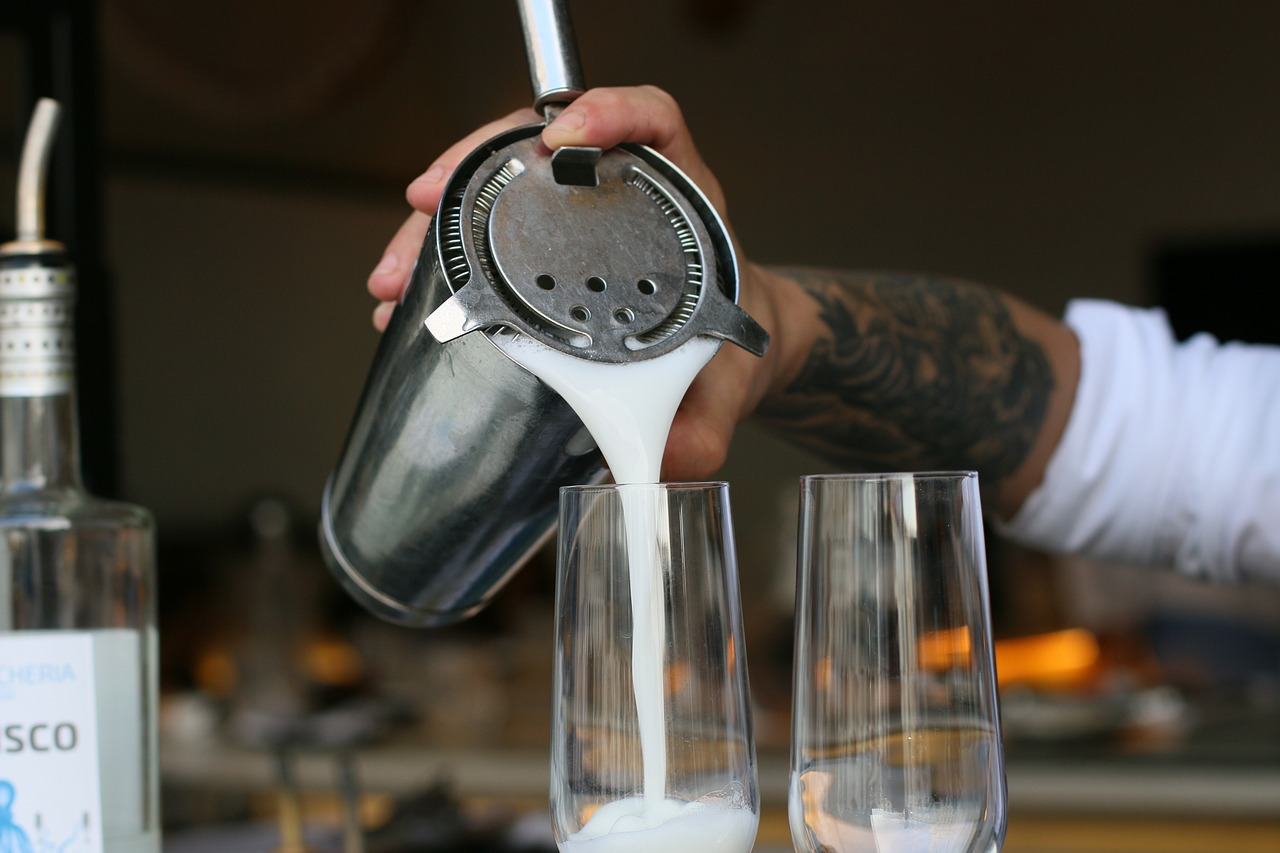
\includegraphics[width=0.25\textwidth]{pisco-sour}
\introduction{
Esta receta la vi por internet. Específicamente en un canal de Insta...
}
\ingredients{
	30 & \unit[ml] de jugo de limón \\
	& Almíbar simple 22.5 \\
	& Clara de huevo 30ml \\
	60 & \unit[ml] de pisco \\
	3 & Gotas de bitter Angostura \\
	& Hielo para enfriar y batir \\
}
\preparation{
    \begin{enumerate}
        \item Verter todo en una coctelera y batir por aproximadamente 10 segundos.
        \item Servir en una copa.
    \end{enumerate}
}
\hint{
Para pasteurizar un huevo, recordar mantener entre 62 a 64 grados máximo, por 4 minutos.
}
\end{recipe}